% brainstorm:

% * citar fundamento em teorias de contornos e pouco uso em composição
% * exemplos das necessidades de operações na composição (peça do mestrado)
% * desenvolvimento do goiaba (para que serve, exemplo de código e de
% saída)
% * trabalhos futuros

\section{Introduction}
\label{sec:introduction}

Contours can be understood as the shape or format of an object. In
Music, contour can be associated to pitch, density, rhythm, intensity,
etc, and represents a parameter in function of another, as pitch in
function of time. For instance, Beethoven's Fifth Symphony main motive
and its contour are represented respectively in figures
\ref{fig:5a-sinfonia-motivo} and \ref{fig:c-3120}.

\begin{figure}[!b]
  \centering
  \subfloat[Main motive]{
    \includegraphics[scale=.9]{5a-sinfonia}
    \label{fig:5a-sinfonia-motivo}
  }

  \subfloat[Contour (3 1 2 0)]{
    \includegraphics{c-3120}
    \label{fig:c-3120}
  }
  \caption{Fifth Symphony main motive contour}
  \label{fig:5a-sinfonia}
\end{figure}

Contour study is important because, like motives and pitch sets,
contours can help to give coherence to a musical piece. Contour can be
aproached by analytical or compositional points of view, and are also
easily recognized by musicians and layman from graphical
representations \cite{marvin88:generalized}.

Contour theories
\cite{friedmann85:methodology,friedmann87:response,morris87:composition,morris93:directions,marvin.ea87:relating,marvin88:generalized,marvin.ea95:generalization,polansky.ea92:possible,quinn97:fuzzy,clifford95:contour,beard03:contour}
provide arrays, matrixes and many operations to help in comparing
contours, like inversion, translation, contour elements comparison,
and contour similarity comparisons, contour interval array, and
comparison matrix.

Contour operations depends on precise mathematical calculations, and
are human errors likely. So a computer program to process contour can
assist composers and analysts in tasks like operations calculation,
minimizing human error; automated graphical plotting; and conversion
from score to contours and vice-versa. For this reason we are
developing \goiaba{}, a contour processor software (see section
\ref{sec:goiaba}).

\section{Contour applications in composition}
\label{sec:cont-appl-comp}

Despite the possible coherence given by contours and the operations
provided by contour theories, systematic studies of contour operations
and combinations usage in musical composition are scarce. For this
reason we are researching contours usage in composition. The first
author of this paper, in his master's\footnote{The reference was
  omitted to keep anonymity. It will be included in final version.},
composed two experimental short pieces and an eleven minutes quintet,
both based in contour theories operations.

\goiaba{} was very important in this quintet compositional process
because the entire piece was composed based on P(5 3 4 1 2 0) contour,
its subsets, operations and combinations. Precise calculations and
graphical representations were required.

For instance, a \eng{fugato}, in the quintet, has subject and
countersubject based on rotation and retrogradation operations. The
subject has original contour P(5 3 4 1 2 0) and factor 3 rotation
(fig. \ref{fig:sujeito-fugato}). The contoursubject has original
contour retrogradation repeated three times with different rotation
factors---5, 4 and 3 (fig. \ref{fig:contra-sujeito-fugato}).

\begin{figure*}
  \centering
  \subfloat[Subject]{
    
\includegraphics[scale=2.8]{sujeito-fugato}
    \label{fig:sujeito-fugato}
  }

  \subfloat[Countersubject]{
    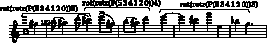
\includegraphics[scale=2.8]{contra-sujeito-fugato}
    \label{fig:contra-sujeito-fugato}
  }
  \caption{Structural elements of \eng{fugato}}
  \label{fig:elementos-fugato}
\end{figure*}

\section{Goiaba}
\label{sec:goiaba}

\goiaba{}\footnote{Additional information and link were also omitted
  to keep anonymity.} is a software developed in Common Lisp
\cite{graham94:lisp}, compiled with Steel Bank Common Lisp (SBCL)
\cite{team07:sbcl}, and bottom up metodology.

Bottom up methodology is related to the development direction, from
simple subsystems to the entire program. This methodology is suitable
to programs that progressively have complexity increased. Programs
like \TeX{}\footnote{\url{www.tug.org}} and X
Windows\footnote{\url{www.x.org}} are developed in this way. This
metodology has good advantages as the possibility to make smaller and
smarter programs, to reuse subsystems functions in others subsystems,
and to simplify and clear programmer ideas \cite{graham94:lisp}.

In \goiaba{}, contours are symbolic represented in two ways: as simple
contours and duration-included contours. Simple contours represents
only contour element values: \code{(5 9 6)}. Duration-included
contours represents also the time when the element occur: \code{((0
  5)(1 9)(2 6))}. Despite \goiaba{} provides a codification that
includes time influence in contour, we don't consider time. It's a
future work (see section \ref{sec:future-work}).

\goiaba{} has \texttt{ponto}, \texttt{contorno-simples} and
\texttt{contorno-duracao} classes. The \texttt{ponto} class defines
pitches in time as (x, y), cartesian elements, x as time and y as
pitch. The \texttt{contorno-duracao} class defines a contour as a
points list, like ((x, y) (z, w)), and the \texttt{contorno-simples}
class defines contours only as pitches, like (y w).

Some read macros were defined to simplify instances making easier. For
instance, to make \texttt{ponto} instance, it's possible to do
\code{(make-instance 'ponto :x 0 :y 3)} or just \code{\#p(0 3)}, with
read macro. It's possible also to create \texttt{contorno-duracao}
with two points in \code{\#d(\#p(0 3) \#p(1 4))}.

Contour operations are implemented in methods, taking Common Lisp
object systems (CLOS) multiple order. So a method like \texttt{rotate}
behaves in a different way depending on the first parameter. In
following code there are two methods, the first to
\code{contorno-duracao}, and the second to \code{contorno-simples}.

%% FIXME: insert code


%% FIXME: update operations
\goiaba{} has many operations to process contours, like inversion,
retrogradation and rotation, contour reduction \cite{adams76:melodic},
contour class, contour adjacency series, contour adjacency series
vector, contour interval, contour interval array, contour class vector
I and II \cite{friedmann85:methodology}, and comparison matrix
\cite{morris93:directions}.

Finally \goiaba{} uses Cl-pdf
library\footnote{\url{www.cliki.net/CL-PDF}} to plot contours,
allowing easy contour operations visualization. For instance, the
follow code generates a graph with original contour, retrogradation,
inversion, and rotation (fig. \ref{fig:operacoes}). In this example we
define \code{Z} contour, output file, graphic dimensions, operations,
and colors to be output in graphic.

%% FIXME: insert code

%% FIXME: insert figure
\begin{figure}
  \centering
  \caption{Z(0 5 3 4 1 3) contour operations}
  \label{fig:operacoes}
\end{figure}

\section{Future work}
\label{sec:future-work}

%%% Local Variables: 
%%% mode: latex
%%% TeX-master: "goiaba-contour-processor"
%%% End: 